\documentclass[UTF8,a4paper,zihao=-4]{ctexart}
\usepackage[left=2.6cm,right=2.6cm,top=2.4cm,bottom=2.5cm]{geometry}
\usepackage{graphicx,amsmath,lmodern,caption}
\usepackage[hidelinks]{hyperref}
\captionsetup{font=small,labelfont=bf,labelsep=quad,skip=7pt}
\setlength{\parindent}{2em}
\setlength{\parskip}{4pt}
\linespread{1.28}
\pagestyle{plain}
\begin{document}
\begin{center}\heiti\Large 图件重设计样稿\end{center}
\noindent\small 本稿按论文版心宽度展示三个候选图及其邻近说明。图内保留必要标识，主要解释放在正文和图注；各图均由本项目已有数值结果绘制。\normalsize

药材内部的含水率分布可以通过中部短段剖切展示。以问题二的 $t=0.5\,\mathrm{h}$ 为例，中心仍接近初始含水率，外层已经下降；此时环境温度高于药材表面温度，水分则由表面向外迁移。图\ref{fig:cutaway}将这两类交换方向与内部径向差异放在同一个几何对象上，使读者先辨认材料、表面与内部的关系，再阅读相应的控制方程和边界条件。

\begin{figure}[htbp]
  \centering
  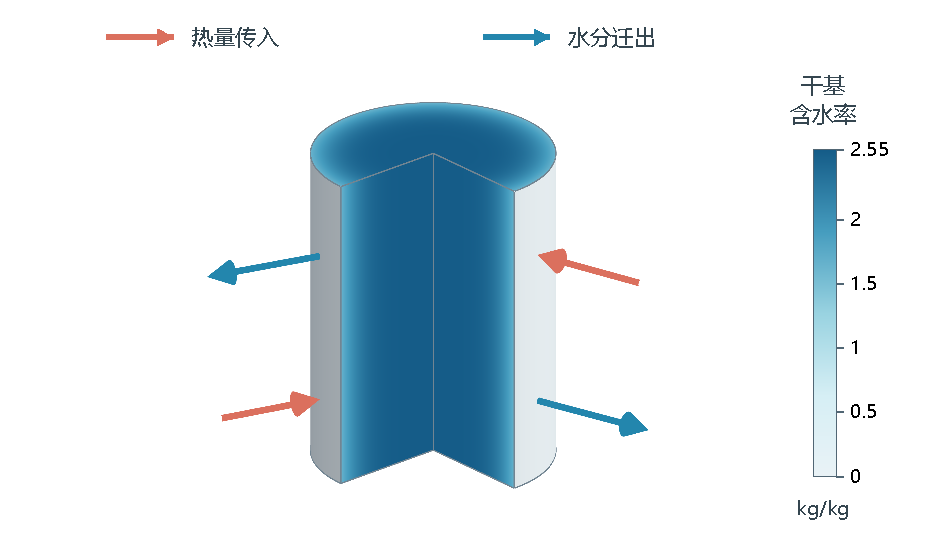
\includegraphics[width=\linewidth]{fig_mechanism_cutaway.pdf}
  \caption{药材中部短段的剖切与表面交换。剖面颜色取问题二 $t=0.5\,\mathrm{h}$ 的干基含水率，箭头表示该时刻热量传入与水分迁出的方向，不表示通量大小。}
  \label{fig:cutaway}
\end{figure}

图中剖切面用于显示已有的一维径向场；沿轴向的延展只是中部短段的示意，不增加轴向求解结果。灰色弧面用于区分外表面与内部剖面，不代表额外的壳层。数值颜色不受照明明暗影响，表面交换方向与该时刻的边界条件一致。

\clearpage
\begin{center}\heiti\large 问题二：温度与含水率的时空变化\end{center}

图\ref{fig:q2}从时间与半径两个方向呈现前三小时的计算结果。温度面上的等值线较为接近竖直，表明升温过程以时间变化为主，同时外层先于中心达到相同温度。含水率面上的等值线则从外层向内推进：相同含水率首先出现在表层，中心下降相对较慢。两个色场的几何差异直接显示了热响应与水分迁移的不同时间尺度，为下一问沿全程轨迹判断干燥终点提供依据。

\begin{figure}[htbp]
  \centering
  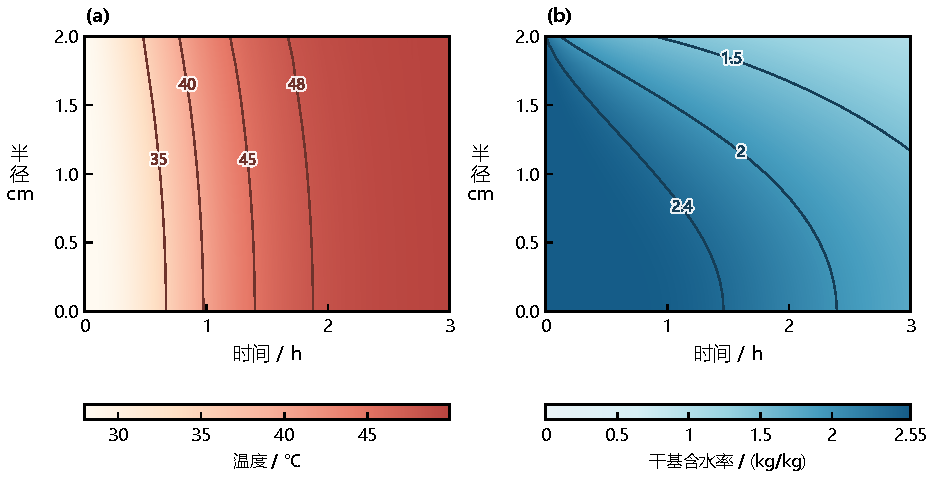
\includegraphics[width=\linewidth]{fig04_q2_fields_sample.pdf}
  \caption{问题二前三小时的时空分布。（a）温度；（b）干基含水率。细线为对应标注值的等值线。色场和等值线依据逐秒保存的21个规定半径值作线性显示内插。}
  \label{fig:q2}
\end{figure}

温度采用暖色，含水率采用蓝色，并各自配置量纲与色标。含水率色标在各图中固定为 $0$ 至 $2.55\,\mathrm{kg/kg}$，因此同一数值不会因图件或时刻不同而改变颜色。图中显示内插仅使已有采样值之间的分布便于阅读，不改变计算结果或宣称新增空间计算精度。

问题三仍应以全程含水率变化及最大值穿越阈值的过程为主图；该图负责说明终点如何判定，无需再承担问题四的收缩几何展示。

\clearpage
\begin{center}\heiti\large 问题四：收缩截面与未达标区域\end{center}

问题四引入半径随时间变化的条件。为将这一特点与前问区分，图\ref{fig:q4}保持相同厘米尺度，绘出六个时刻的截面。前期变化同时体现在外轮廓缩小与含水率下降；后期外半径已基本稳定，内部尚未达标的区域仍在缩小。由此可见，外形接近稳定并不能替代全域含水率判据。

\begin{figure}[htbp]
  \centering
  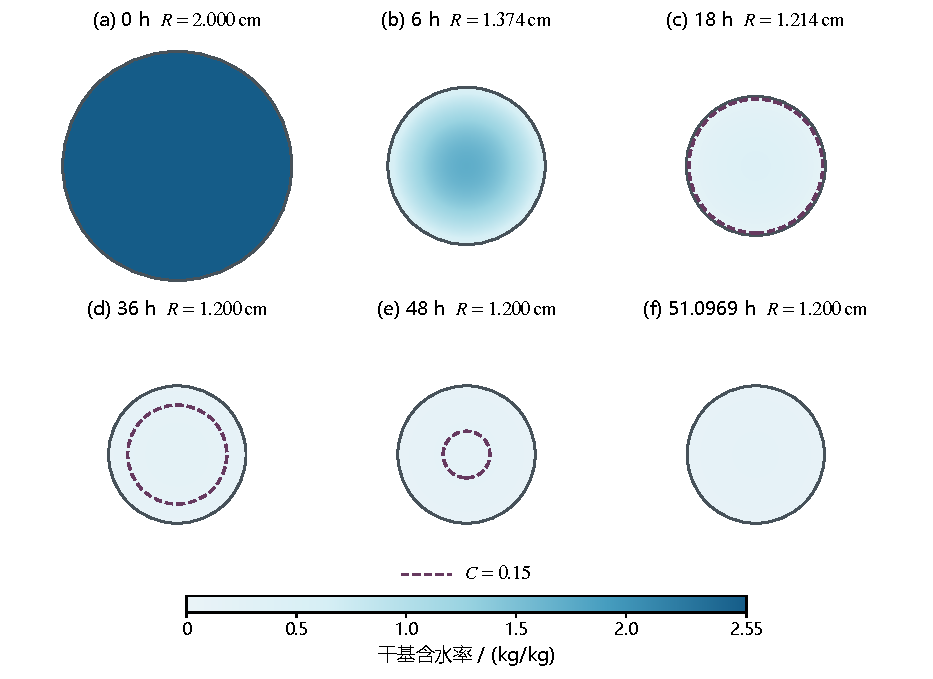
\includegraphics[width=\linewidth]{fig07_q4_sections_sample.pdf}
  \caption{问题四的同尺度含水率截面序列。实线为实际外表面，紫色虚线为 $C=0.15\,\mathrm{kg/kg}$ 等值线。截面由各时刻完整径向场按 $r=R(t)\xi$ 绘制，统一使用同一线性色标。}
  \label{fig:q4}
\end{figure}

在出现虚线的三个时刻，其内侧对应尚未达标的区域；初始和 $6\,\mathrm{h}$ 时整个截面均未达标。最后一幅取首个严格达标整数秒 $183949\,\mathrm{s}$，此时全部保存节点的未舍入含水率均低于 $0.15\,\mathrm{kg/kg}$，因而不再出现阈值内圈。虚线是数值等值线，不作相界面的解释；截面大小表示几何尺度，不能直接当作水质量。

这一图形侧重说明“尺寸变化”与“内部达标过程”的关系。精确的终点比较及数值误差仍由邻近表格与模型检验承担，图内不堆放说明段落。
\end{document}
